\RequirePackage[l2tabu, orthodox]{nag}
\documentclass[11pt, english]{article}
\usepackage{mathtools}
\usepackage{amssymb,amsmath}
%\usepackage{fullpage}
\usepackage[margin=0.9in]{geometry}
\usepackage{setspace}
\parskip 10pt
\usepackage{tikz}
\linespread{1.6}
\usepackage{enumitem}
\usepackage{parskip}
\usepackage{pdfpages}
\usepackage{graphicx}   % For including images
\usepackage{subcaption} % For subfigures and captions
\usepackage[justification=centering]{caption} 
\usepackage{multirow}
\usepackage{float}
\usepackage[english]{babel}
\usepackage[toc,page]{appendix}
\usepackage{pdflscape}
\usepackage{array}
\usepackage{booktabs}
\usepackage{hyperref}
\hypersetup{colorlinks=true, urlcolor=blue, linkcolor=black}
\usepackage{microtype}
\title{APS360}
\author{Ziyue Jin}
\date{Winter 2025}

\begin{document}

\maketitle
\newpage
\section{Lecture01}
\subsection{Deep learning}
The latest version of Artificial Neural Networks or Connectionism(old ML method).
Thresholded logic unit 1943, Perception 1957, adaline 1960, XOR problem 1969, Multilayer backprop 1982, CNNs 1989, LSTMs 1997, SVMs 1995, Deep Nets 2006, Alex net 2012.

\subsection{Types of Biases}
\textbf{Inductive bias} can be defined as the set of assumptions or biases that a learning algorithm employs to make predictions on unseen data based on its training data. These assumptions are inherent in the algorithm's design and serve as a foundation for learning and generalization.
\textbf{Reporting bias.} This type of AI bias arises when the frequency of events in the training dataset doesn’t accurately reflect reality. 
\textbf{Selection bias. }This type of AI bias occurs if training data is either unrepresentative or is selected without proper randomization.  
\textbf{Group attribution bias} takes place when data teams extrapolate what is true of individuals to entire groups the individual is or is not part of.  
\textbf{Implicit bias.} This type of AI bias occurs when AI assumptions are made based on personal experience that doesn’t necessarily apply more generally.  

\subsection{Supervised Learning}
\begin{itemize}
    \item Regression or classification.
    \item Requires data with ground truth labels and outputs.
\end{itemize}
Models learn to maps an input to an output based on example input-output pairs.
\subsubsection{Classification}: This algorithm helps to predict a discrete value. It can be thought, the input data as a member of a particular class or group. 
\begin{itemize}
    \item Naive Bayes Classifier
    \item Support Vector Machines
    \item Logistic Regression
\end{itemize}
\subsubsection{Regression}: These problems are used for continuous data. For example, predicting the price of a piece of land in a city, given the area, location, number of rooms, etc.  
\begin{itemize}
    \item Linear Regression
    \item Nonlinear Regression
    \item Bayesian Linear Regression
\end{itemize}
\[y(x, \mathbf{w}) = w_0 + w_1x + w_2x^2 + \dots + w_Mx^M = \sum_{j=0}^{M} w_jx^j
\]
\subsubsection{Loss Function}: The cost of each perdictive function.  Learn a mapping between input features (x) and output labels (y).
\[E(\mathbf{w}) = \frac{1}{2} \sum_{n=1}^{N} \left\{ y(x_n, \mathbf{w}) - t_n \right\}^2
\]

 \subsection{Unsupervised Learning}
 \begin{itemize}
     \item Self-supervised learning, semi-supervised learning.
     \item Requires observations without humans annotations.
 \end{itemize}
No complete and clean labelled dataset in unsupervised learning. It is self-organized learning. Its main aim is to explore the underlying patterns and predict the output.  
\begin{itemize}
    \item K – Means clustering
    \item Neural Networks
    \item Principal Component Analysis
\end{itemize}
\subsubsection{Loss Function}: Discover patterns, clusters, or representations in data without labeled outputs. 
\subsection{Reinforcement Learning}
\begin{itemize}
    \item Sparse rewards form environment(won/lost).
    \item Actions affects the environment(dynamic).
\end{itemize}
The algorithms learn to react to an environment on their own.  

\subsection{Fitting}
Cannot use all data for training, needs to use some to test the model. 
\subsubsection{\textbf{Avoid Overfitting}}
Occurs when a model learns not only the underlying patterns in the training data but also the noise and random fluctuations. This results in \textbf{excellent performance on the training data} but \textbf{poor generalization to unseen or test data}.
More data helps the model to learn better and generalize better.
\begin{enumerate}
    \item \textbf{Regularization}:
    \begin{itemize}
        \item Add penalties to large weights in the loss function.
        \item Example (L2 Regularization): 
        \[
        \text{Loss} = \text{Original Loss} + \lambda \sum w^2
        \]
        \item Encourages smaller weights, reducing model complexity.
    \end{itemize}
    
    \item \textbf{Simplify the Model}:
    \begin{itemize}
        \item Use fewer layers or nodes in a neural network.
        \item Select a simpler algorithm (e.g., linear regression instead of high-degree polynomial regression).
    \end{itemize}
    \item \textbf{Increase Training Data}:
    \begin{itemize}
        \item Collect more labeled examples to improve the model's ability to generalize.
    \end{itemize}
    \item \textbf{Data Augmentation}:
    \begin{itemize}
        \item Apply transformations such as flipping, rotating, or cropping images to artificially increase the dataset size.
    \end{itemize}
    \item \textbf{Cross-Validation}:
    \begin{itemize}
        \item Use techniques like $k$-fold cross-validation to ensure consistent performance across different subsets of data.
    \end{itemize}
    \item \textbf{Early Stopping}:
    \begin{itemize}
        \item Stop training when validation performance stops improving, even if training performance continues to improve.
    \end{itemize}
    \item \textbf{Dropout (Neural Networks)}:
    \begin{itemize}
        \item Randomly deactivate a fraction of neurons during each forward pass to prevent co-dependency among features.
    \end{itemize}
    \item \textbf{Reduce Noise in Data}:
    \begin{itemize}
        \item Remove irrelevant features or outliers in the dataset.
    \end{itemize}
\end{enumerate}

\subsection{Artificial Neuron}
$x_i$ - the input such as a pixel in an image.
$w_i$ - the weight of input $x_i$.
b - the bias, weight with no input.
f - the activation function that determines how our output changes with the sum of all weight-input products.
y - the output such as the class an image belongs to.
\[y_p = f(w\times x+b)\]
\subsection{Activation Functions}
\subsubsection{Sign Function}
\[f(x) = sign(x)\]
\subsubsection{Heaviside(unit) step function}
\[f(x) =
\begin{cases} 
0, & \text{if } x < 0 \\
1, & \text{if } x \geq 0
\end{cases}\]
These are called decision boundaries. Not differential, continuous or smooth.

\subsubsection{Sigmoid Activation Function}
\begin{itemize}
    \item Easily differentiable, smooth, continuous.
    \item Range between [-1, 1] or [0, 1].
    \item Gradients become vanishingly small very quickly away from x=0.
\end{itemize}
\[f(x) = tanh(x)\]
\[f(x) = \frac{1}{1+e^{-x}}\]
\subsubsection{ReLU Activation Function}- Rectified Linear Unit
\subsubsection*{ReLU}
\[
\text{ReLU}(x) = (x)^+ = \max(0, x)
\]

\subsubsection*{Leaky ReLU}
\[
\text{LeakyReLU}(x) = 
\begin{cases} 
x, & \text{if } x \geq 0, \\
\text{negative\_slope} \times x, & \text{otherwise.}
\end{cases}
\]

\subsubsection*{Parametric ReLU}
\[
\text{PReLU}(x) = 
\begin{cases} 
x, & \text{if } x \geq 0, \\
a x, & \text{otherwise.}
\end{cases}
\]

\section{Lecture02}
\subsection{Loss Function}
\subsubsection{Softmax}
Normalizes the logics into a categorical probability distribution  of all possible classes.
The sum of the possibilities = 1.
\subsubsection{One-hot encoding}
Maps categories to a vector representation. (ie. ECE253 state machines)
\subsubsection{Mean Squared Error(MSE)}
Mostly used for regression problems.
\[x_i = (p_i - t_i)^2\]
\[x_i = i^{th} MSE , p_i = predicted, t_i = ground \]
\subsubsection{Cross Entropy(CE)}
Mostly used for classification problems
\[
\text{CE} = -\frac{1}{N} \sum_{n=1}^{N} \sum_{k=1}^{K} t_{n,k} \log(y_{n,k})
\]
\subsubsection*{Binary Cross-Entropy Loss}
\[
\text{BCE} = -\frac{1}{N} \sum_{n=1}^{N} \left[ t_n \log(y_n) + (1 - t_n) \log(1 - y_n) \right]
\]

\subsection{Gradient Decent}
Learning rate window 0.1-0.0001.\\
Adjusting weights according to the gradient gives a max/min error learning rate times.
\begin{figure}[H]
    \centering
        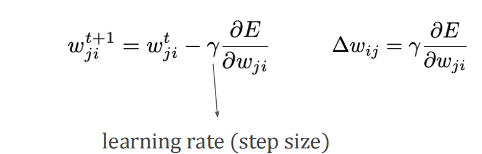
\includegraphics[width=0.5\linewidth]{image.png}
    \caption{derivative of the error to change of weight. (rate*velocity)}
    \label{fig:enter-label}
\end{figure}
\textbf{Training Sample}
\begin{figure}[H]
        \centering
        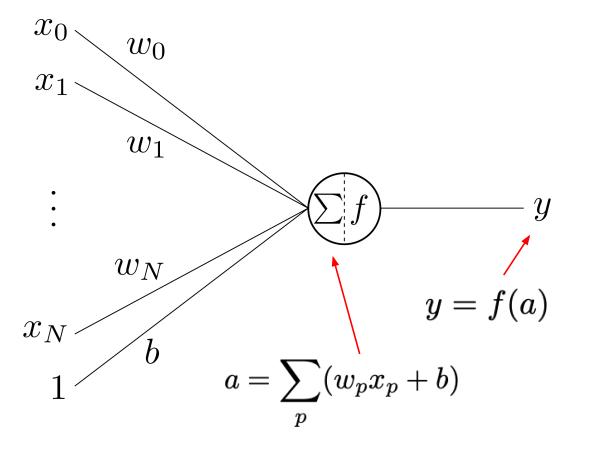
\includegraphics[width=0.5\linewidth]{Screenshot 2025-01-14 at 7.40.24 PM.png}
        \caption{Delta Rule for Single Weight}
        \label{fig:enter-label}
\end{figure}
Use the chain rule to find $\frac{dE}{dw_p}$
\begin{equation}
    E = (y-t)^2, f(x) = \frac{1}{1+e^{-1}}
\end{equation}
Then Use the chain rule to find $\frac{dE}{dw_p}$
\[
\frac{dE}{dw_p} = \left( \frac{dE}{dy} \right) \left( \frac{dy}{da} \right) \left( \frac{da}{dw_p} \right)
\]

\[
\frac{dE}{dy} = \frac{d\left( (y - t)^2 \right)}{dy} = 2(y - t)
\]

\[
\frac{dy}{da} = \frac{d\left( \frac{1}{1 + e^{-a}} \right)}{da} = (1 - y)y
\]

\[
\frac{da}{dw_p} = x_p
\]
\[
\frac{dE}{dw_p} = 2(x_p)((y - t)((1 - y)(y)))
\]

\subsubsection{Forward and Backward-Pass}
\begin{figure}
    \centering
    \includegraphics[width=0.5\linewidth]{sample code}
    \caption{Sample Code (Updates Weight)}
    \label{fig:enter-label}
\end{figure}
\subsection{Neural Network Architectures}
\begin{itemize}
    \item Complex operations need multiple layers to calculate.
    \item XOR function needs at least one hidden neural network layer. 
\end{itemize}
 \begin{figure}[H]
     \centering
     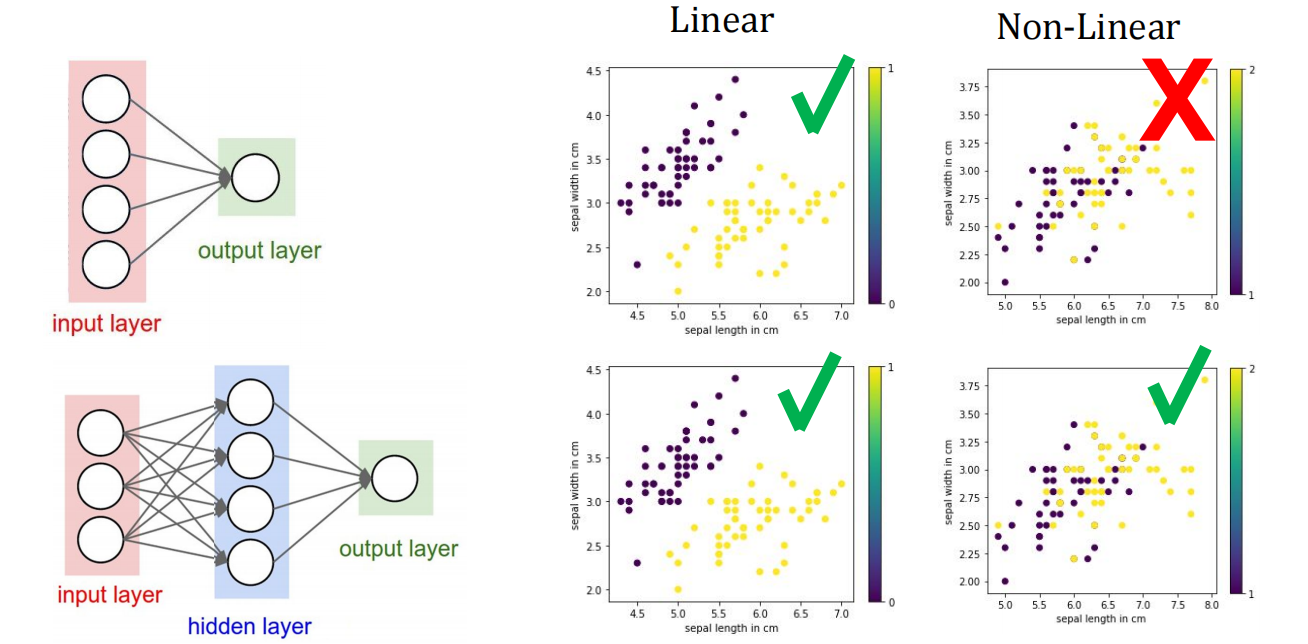
\includegraphics[width=0.7\linewidth]{Screenshot 2025-01-14 at 7.49.26 PM.png}
     \caption{Multiple Layers with Non-Linearity}
     \label{fig:enter-label}
 \end{figure}
 Layers use activations of the previous layer as high-level features representing the input data(intermediate).
 The goal for the final layer is a\textbf{ linear separation.}
 \begin{itemize}
     \item Feed-Forward Network: Information only flows in one direction(one dimensional) from input to output.
     \item Fully-Connected Network: Neurons between adjacent layers are fully connected. All neurons from previous layers connect to the current layer, all the weights are present.
     \item Number of Layers = Number of hidden layers + output layer.
 \end{itemize}
 \begin{figure}[H]
     \centering
     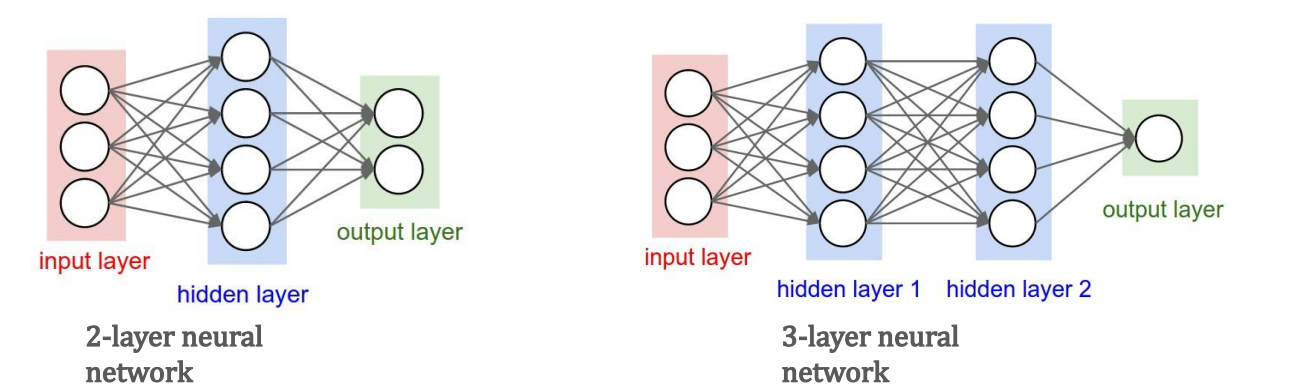
\includegraphics[width=0.7\linewidth]{Screenshot 2025-01-14 at 7.55.37 PM.png}
     \caption{Layered Neural Network (Fully Connected}
     \label{fig:enter-label}
 \end{figure}
\subsection{Universal Approximation Theorem:}
The theorem states that a feedforward neural network with \textbf{a single hidden layer} containing a sufficient number of neurons and a suitable non-linear activation function can approximate any continuous function on a compact input domain to any desired accuracy.

 \section{Lec03}
\subsection{Hyper Parameters}
weight = 1*number of columns in data,  updated through gradient descent (Inner loop of optimization).
labels = 1*number of rows in data
Batch size = number of groups
Number of layers = n input layers + n output layer
Layer size = dimension of the layer
Type of activation function
Learning rate
\begin{figure}
    \centering
    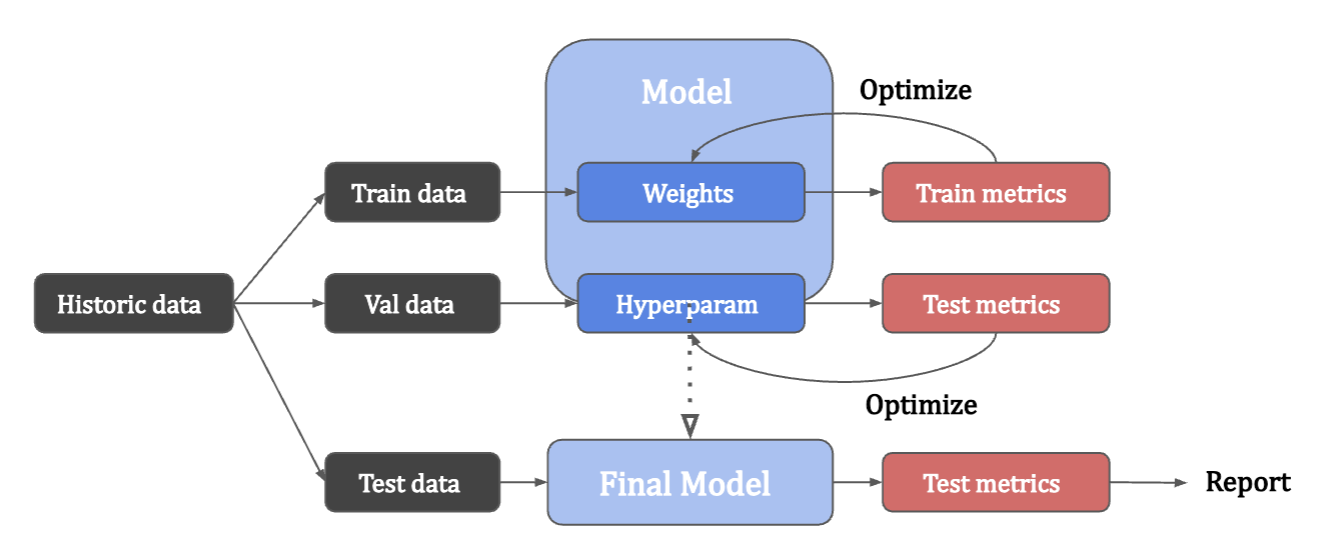
\includegraphics[width=0.5\linewidth]{Screenshot 2025-02-04 at 3.41.17 PM.png}
    \caption{Stratified Sampling
without Replacement}
    \label{fig:enter-label}
\end{figure}
\subsection{Stochastic Gradient Descent(SGD)}
In SGD, instead of using the entire dataset for each iteration, only a single random training example (or a small batch) is selected to calculate the gradient and update the model parameters. This random selection introduces randomness into the optimization process.
\textbf{Advantage: }computational efficiency, especially when dealing with large datasets.
\textbf{Note:} generally noisier than typical Gradient Descent, it usually took a higher number of iterations to reach the minima, because of the randomness in its descent.
\subsection{SGD with Momentum}
Increases for dimensions whose gradients point in the same direction and reduces updates for dimensions whose gradients change directions. Avoids fluctuations around ravines.
\[
\begin{cases}
v_{ji}^t = \lambda v_{ji}^{t-1} - \gamma \frac{\partial E}{\partial w_{ji}} \\
w_{ji}^{t+1} = w_{ji}^t + v_{ji}^t
\end{cases}
\]
\subsection{Adaptive Moment Estimation(Adam)}
Each weight has its own rate
\begin{itemize}
    \item Rapid convergence
    \item Requires minimal tuning
    \item Commonly used
\end{itemize}
\subsection{Auxiliary loss}
Is an additional loss besides the main branch loss to help optimize the learning process of the neural net- works. 
\subsection{Mini-Batch Gradient Descent}
 divides the training data into small subsets called mini-batches, allowing the model to update its parameters more frequently compared to using the entire dataset at once.
Instead of updating weights after calculating the error for each data point  or after the entire dataset, mini-batch gradient descent updates the model’s parameters after processing a mini-batch of data. This provides a balance between computational efficiency and convergence stability.
\textbf{Advantages: }improve both the computational efficiency and the convergence rate of the training process.
\begin{enumerate}
    \item Image Classification
    \item Natural Language Processing (NLP)
    \item Generative Models
\end{enumerate}
\subsection{Batch Size}
Small: 
\begin{itemize}
    \item will optimize a different function loss at each iteration
    \item noisy
\end{itemize}
Large:
\begin{itemize}
    \item expensive
    \item average loss might not change very much as the batch size grows
    \item larger not always better
\end{itemize}
\subsection{Learning Rate}
 the learning rate defines the size of each optimizer's step during each iteration. 
 Larger step size = bigger change in parameters.
 Depends on the learning problem, the optimizer, the batch size and stage of learning.
\subsection{Normalization}
\subsubsection{Batch Normalization}: higher learning rate, regulates the model, less sensitive to initialization. It depends on batch size(not effective on small batches), and cannot work with SGD.
\subsubsection{Layer Normalization}: No moving average or parameters, easy implementation, not dependent on batch size. 
\subsection{Dropout}
The practice of disregarding certain nodes in a layer at random during training. Dropout regularization in deep learning is a regularization approach that prevents overfitting by ensuring that no units are codependent with one another. \\
\textbf{During training - }drop activations with probability p
\textbf{During inference -} multiply weights by (1-p) to keep the same distribution.
\subsection{Weight Decay}
Prevents the weights form growing too fast, lowers variance. Multiplicative proportional to W.
\[
E(W; y, t) = E(W; y, t) + \frac{\alpha}{2} \| W \|_2^2 \xrightarrow{\frac{\partial E}{\partial W}} \frac{\partial E}{\partial W} = \frac{\partial E}{\partial W} + \alpha W
\]

\[
W_{t+1} = W_t - \gamma \left( \alpha W_t + \frac{\partial E}{\partial W} \right)
\]
\subsection{Early Stopping with Patience}
In each training iteration, observe the validation loss\\
As soon as validation loss starts to increase, start a counter\\
If the validation loss decreases, reset the counter\\
Otherwise, wait for a fixed iterations (patience) and then stop the training
\begin{figure}
    \centering
    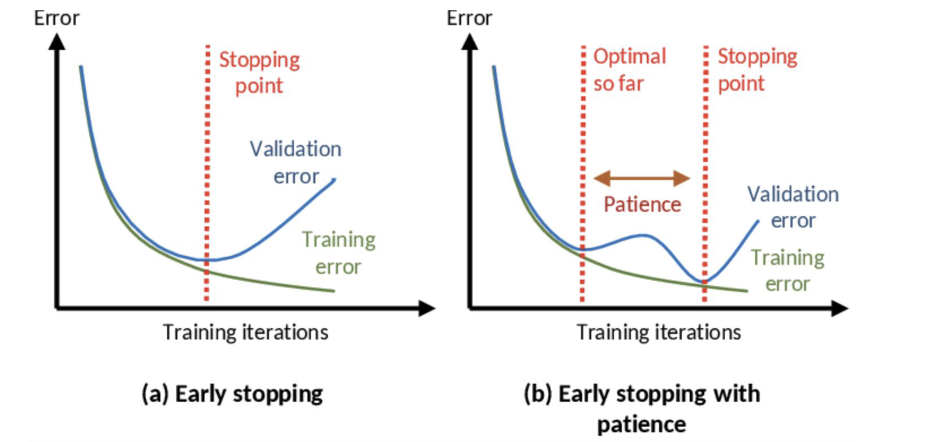
\includegraphics[width=0.5\linewidth]{Screenshot 2025-01-22 at 3.41.54 PM.png}
    \caption{Enter Caption}
    \label{fig:enter-label}
\end{figure}
\subsection{Pytorch}
\begin{figure}[H]
    \centering
    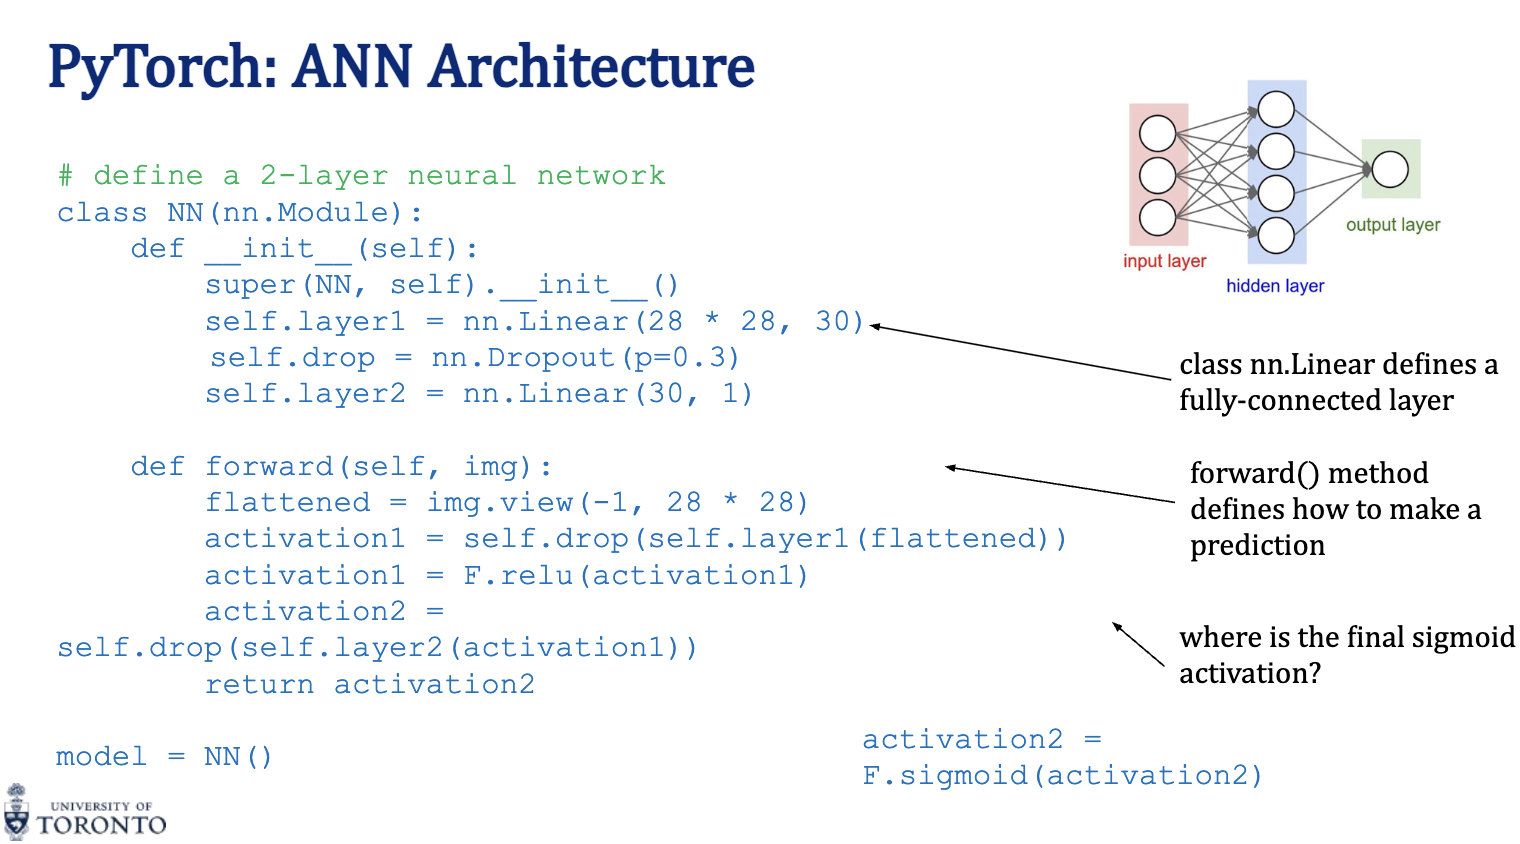
\includegraphics[width=0.5\linewidth]{Screenshot 2025-01-22 at 3.58.15 PM.png}
    \caption{2-Layer Neural Network}
    \label{fig:enter-label}
\end{figure}
\subsection{Forward and Backward Pass in Neural Networks}
\begin{itemize}
    \item \textbf{Forward pass: makes a prediction}
    \begin{itemize}[label=\(\circ\)]
        \item e.g., \texttt{model(input)}, which calls \texttt{network.forward} method
        \item Information flows forwards from input to output layer
    \end{itemize}
    \item \textbf{Backward pass: computes gradients for making changes to weights}
    \begin{itemize}[label=\(\circ\)]
        \item e.g., \texttt{loss.backward()}
        \item Information flows backwards from output to input layer
    \end{itemize}
\end{itemize}
\subsection{Loss Function and Final Activation}
criterion = nn.BCELoss()
\begin{itemize}
    \item Inputs are from a Bernoulli distribution.
\end{itemize}
criterion = nn.BCEWith LogitsLoss()
\begin{itemize}
    \item Applies sigmoid activation internally.
    \item Inputs can be raw logits (unnormalized scores) and do not need to be passed through a sigmoid.
\end{itemize}
\begin{figure}[H]
    \centering
    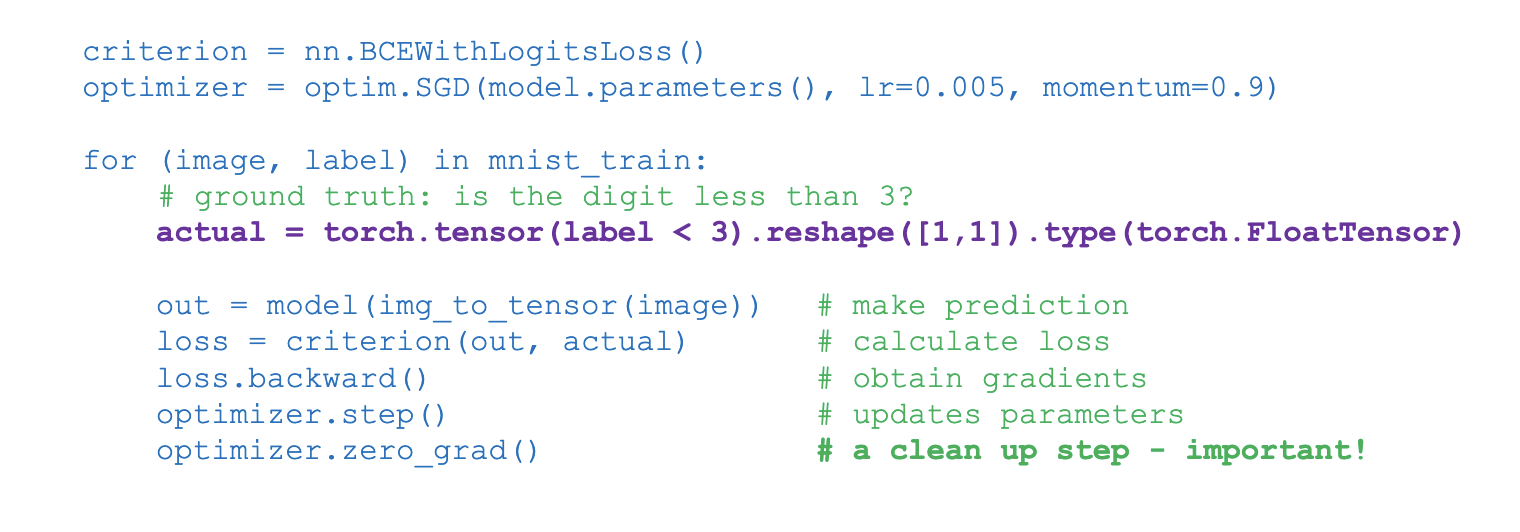
\includegraphics[width=0.75\linewidth]{Screenshot 2025-01-22 at 4.02.25 PM.png}
    \caption{Training code for binary classification problem}
    \label{fig:enter-label}
\end{figure}
\subsection{Multi-Class Classification}
\begin{itemize}
    \item The final output layer has as many neurons as classes.
    \item Apply the softmax activation function on the final layer to obtain class probabilities.
    \item Use the multi-class cross-entropy.
\end{itemize}
\subsection{Loss Function and Final Activation}
criterion = nn.NLLLoss()
\begin{itemize}
    \item Inputs are from a categorical distribution.
\end{itemize}
criterion = nn.CrossEntropyLoss()
\begin{itemize}
    \item Inputs are logits.
    \item Applies softmax activation internally.
\end{itemize}
\begin{figure}
    \centering
    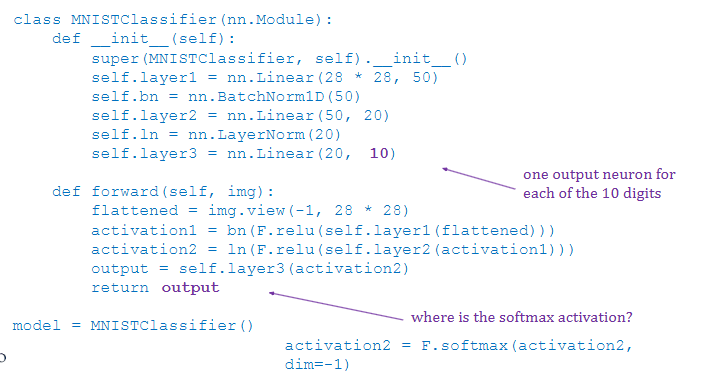
\includegraphics[width=0.75\linewidth]{multiclass.png}
    \caption{Multi-Class ANN Architect}
    \label{fig:enter-label}
\end{figure}
\subsection{Output Probabilities}
\subsection{Measurement of Model Performance}
\begin{enumerate}
    \item \textbf{Precision:}
\begin{itemize}
    \item Measures the proportion of true positives among all positive predictions.
    \item Useful when false positives are costly.
\end{itemize}
    \item \textbf{Recall (Sensitivity):}
\begin{itemize}
    \item Measures the proportion of true positives among all actual positives.
    \item Useful when false negatives are costly.
\end{itemize}
    \item \textbf{F1-Score:}
\begin{itemize}
    \item Harmonic mean of precision and recall, balancing both metrics.
\end{itemize}
    \item \textbf{ROC-AUC (Receiver Operating Characteristic - Area Under Curve):}
\begin{itemize}
    \item Evaluates the model's ability to distinguish between classes.
\end{itemize}
    \item \textbf{Confusion Matrix:}
\begin{itemize}
    \item Provides a detailed breakdown of true positives, true negatives, false positives, and false negatives.
\end{itemize}
\end{enumerate}

prob= F.softmax(output, dim=1)
\begin{figure}
    \centering
    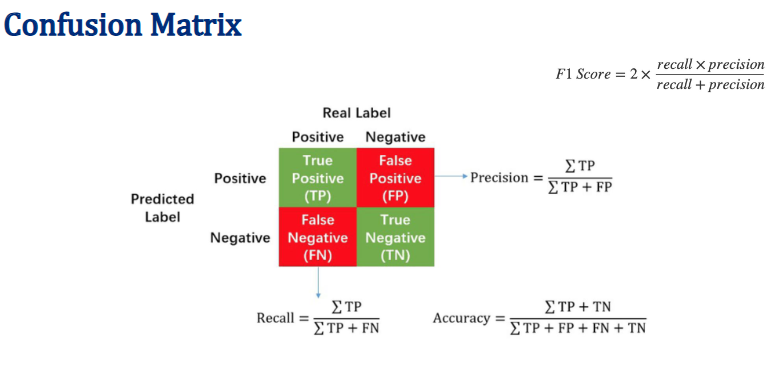
\includegraphics[width=0.75\linewidth]{ConfusionMatrix.png}
    \caption{Confusion Matrix}
    \label{fig:enter-label}
\end{figure}
\section{Lec04}
\subsection{Large Fully Connected Network}
\textbf{Computational complexity} grows, harder to train, and more data to generalize.
Bad\textbf{ inductive bias}, ignores geometry on image data.
\textbf{Not flexible}, different image sizes require different models.
\subsection{Convolution operator in one-dimension}
A mathematical operation on two functions that expresses how the shape of one is modified by the other.
\begin{figure}[H]
    \centering
    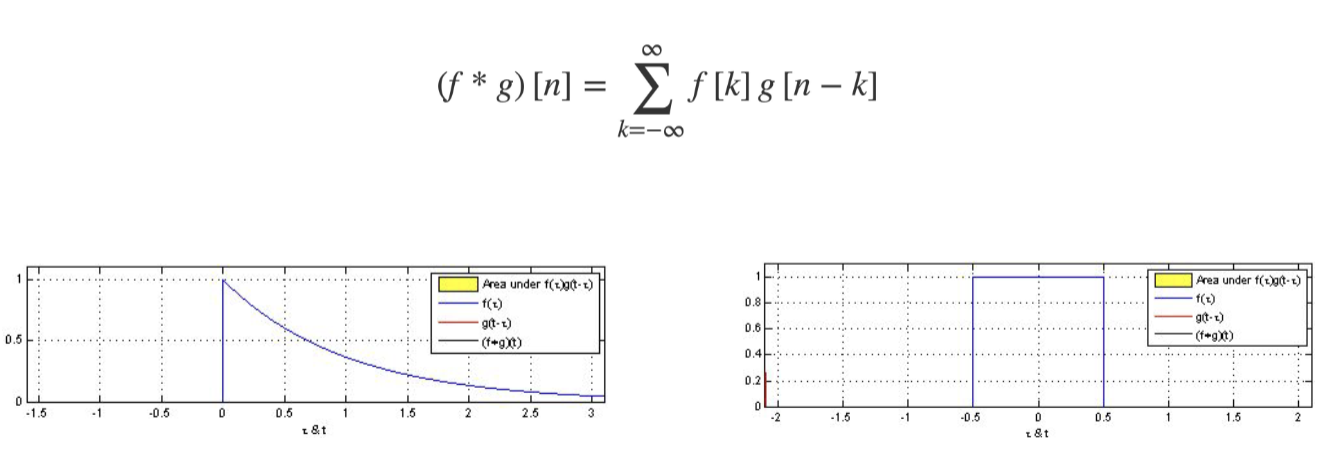
\includegraphics[width=0.7\linewidth]{convolution.png}
    \caption{Convolution operator}
    \label{fig:enter-label}
\end{figure}
\subsection{Convolution Operator in two-dimension}
Convolution of Image I with filter kernel K
\begin{itemize}
    \item Multiply each pixel in I in the range of kernel by the corresponding element of kernel
    \item Sum all these products and write to a new 2d array
    \item Slide kernel across all areas of the image until you reach the ends.
    The resulting shape corresponds to how many times the filter moves in which direction.
\end{itemize}
\begin{figure}[H]
    \centering
    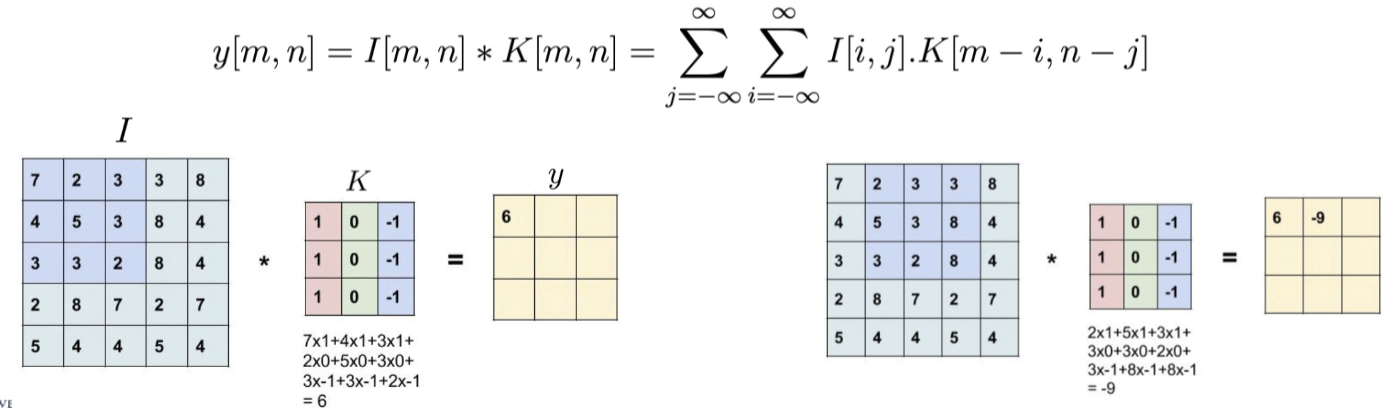
\includegraphics[width=0.8\linewidth]{kernel.png}
    \caption{Convolution in 2D for images}
    \label{fig:enter-label}
\end{figure}
\begin{figure}[H]
    \centering
    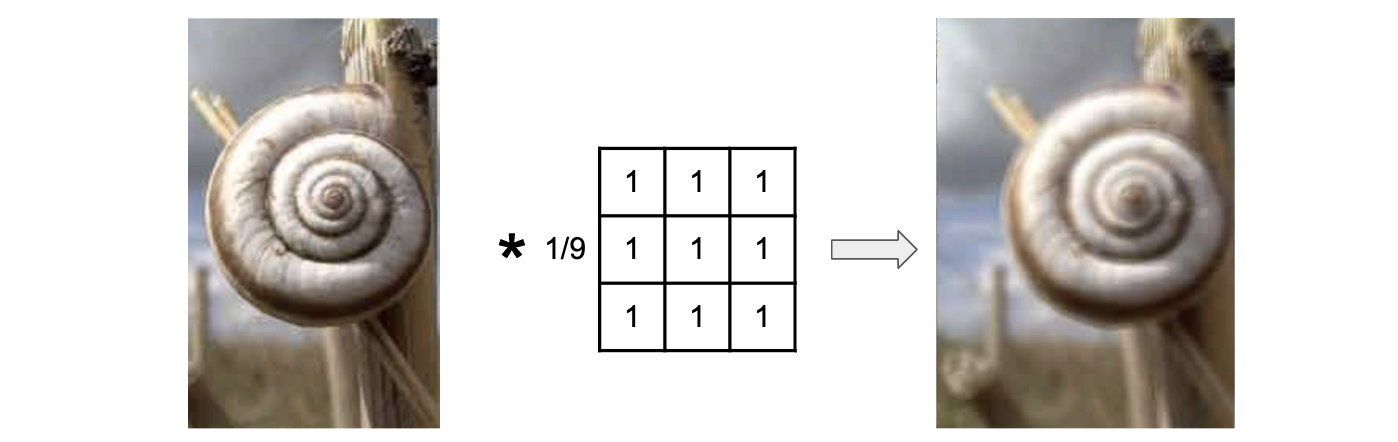
\includegraphics[width=0.7\linewidth]{blurry.png}
    \caption{Blurry Kernel}
    \label{fig:enter-label}
\end{figure}
Horizontal/vertical edge detector (Horizontal/vertical line of 0s).
These kernels used to be hand-crafted.
Classical computer vison: Classic computer vision → multi-stage feature (kernel) engineering.
\subsection{Convolutional Neural Networks}
\textbf{Multilayer Perception(MLP): }
\begin{itemize}
    \item Requires that we pre-process the input.
\end{itemize}
\textbf{Convolutional Neural Network(CNN): }
\begin{itemize}
    \item Apply convolution to image tensors.
    \item The weight sharing occurs across all spatial dimensions.
\end{itemize}
\begin{figure}
    \centering
    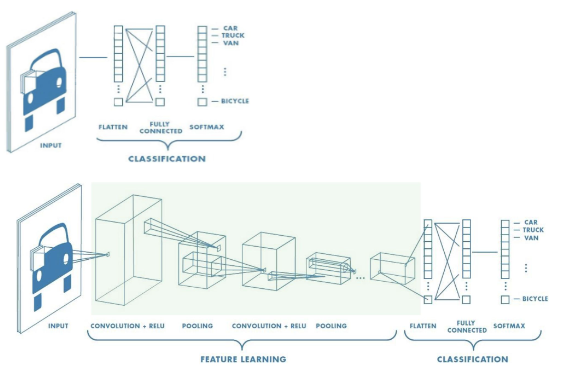
\includegraphics[width=0.75\linewidth]{MLPCNN.png}
    \caption{MLP vs CNN}
    \label{fig:enter-label}
\end{figure}
\subsection{Forward and Backward Pass}
Initialize the kernels randomly 
\textbf{Forward:} Convolve the image with the kernel.
\textbf{Backward:} Update the kernel using gradients.
\subsection{Stride}
Distance between two consecutive positions of the kernel
\begin{itemize}
    \item Allows us to control the output resolution.
\end{itemize}
\subsection{Zero Padding}
Adding zeros around the border of the image before convolution
\begin{itemize}
    \item Keep width and height consistent withe the previous layer.
    \item Keep the information around the border of the image.
\end{itemize}
\subsection{Computing the Output Size}
The size of the output dimension is computed by 
\[
o = \frac{i+2p-k}{s}+1
\]
\begin{itemize}
    \item Image dimension of size i
    \item Kernal of size k
    \item Padding of size p
    \item Stride of size s
\end{itemize}
\subsubsection{Advantages}
\begin{enumerate}
    \item they are more efficient by sharing weights.
    \item they don’t depend on the input image size.
    \item they use geometric information within the images.
\end{enumerate}
\begin{figure}[H]
    \centering
    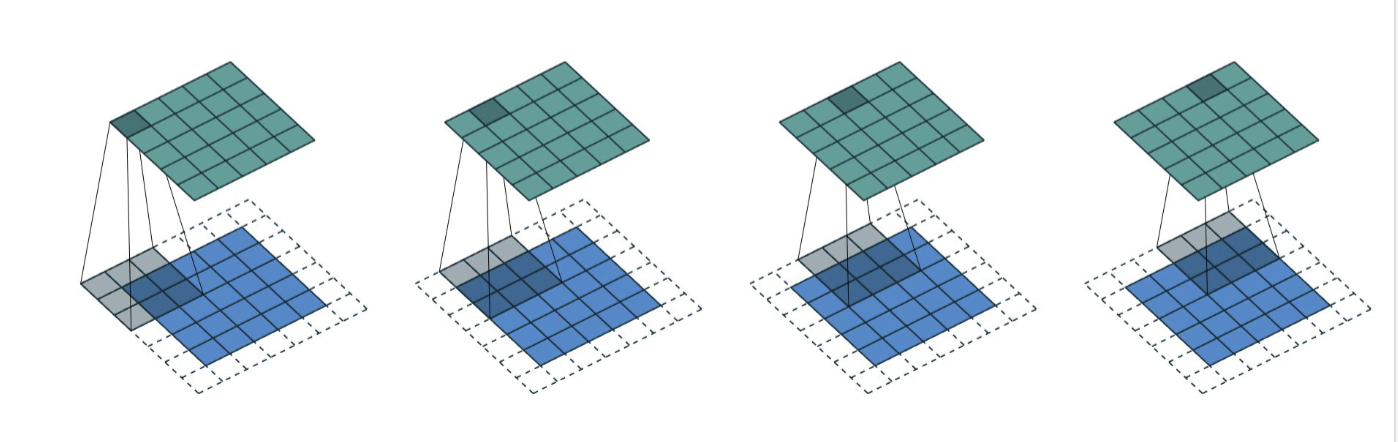
\includegraphics[width=0.75\linewidth]{Zero Padding.png}
    \caption{Zero Padding}
    \label{fig:enter-label}
\end{figure}
\begin{figure}[H]
    \centering
    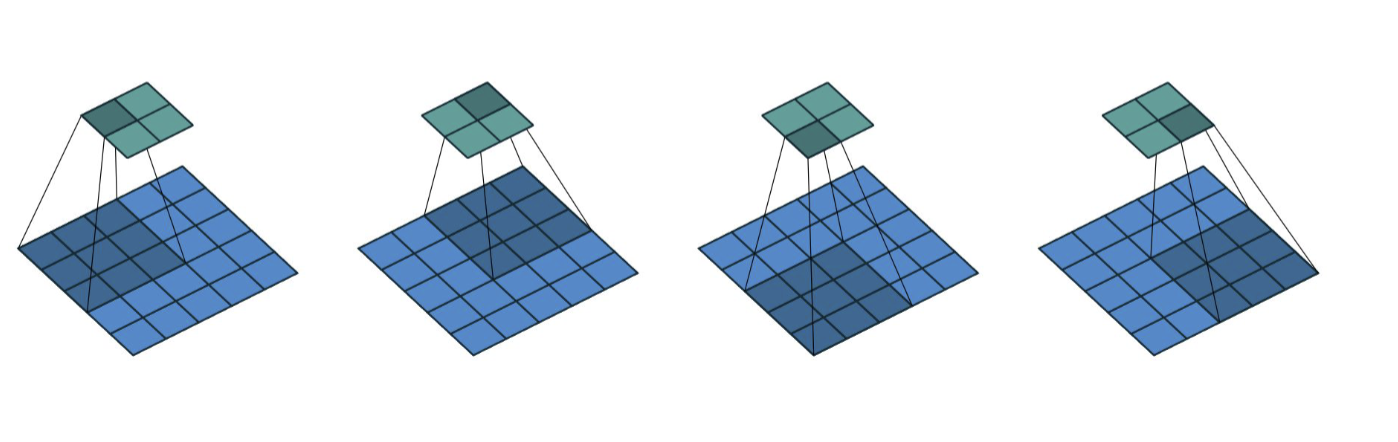
\includegraphics[width=0.75\linewidth]{Screenshot 2025-01-28 at 7.10.53 PM.png}
    \caption{Stride}
    \label{fig:enter-label}
\end{figure}
\subsection{RGB}
Kernel dim = 3*k*k,
Image dim = 3*i*i.\\
\textbf{Example:}
Color input image:3*28*28
Convolution kernel: 3*3*3
Trainable weights: 27
Bias: 1
Parameter: 28
assign more kernels to detect more features\\
\begin{figure}[H]
    \centering
    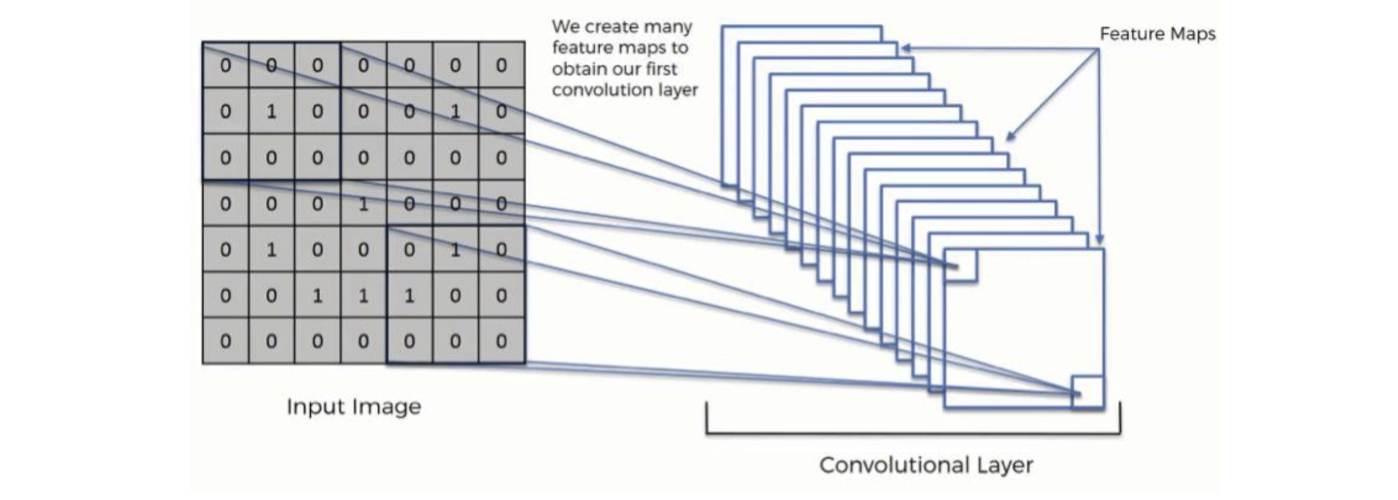
\includegraphics[width=0.75\linewidth]{Screenshot 2025-01-28 at 7.24.16 PM.png}
    \caption{Expanding Feature Maps}
    \label{fig:enter-label}
\end{figure}
Keeping each layers separated
\begin{figure}[H]
    \centering
    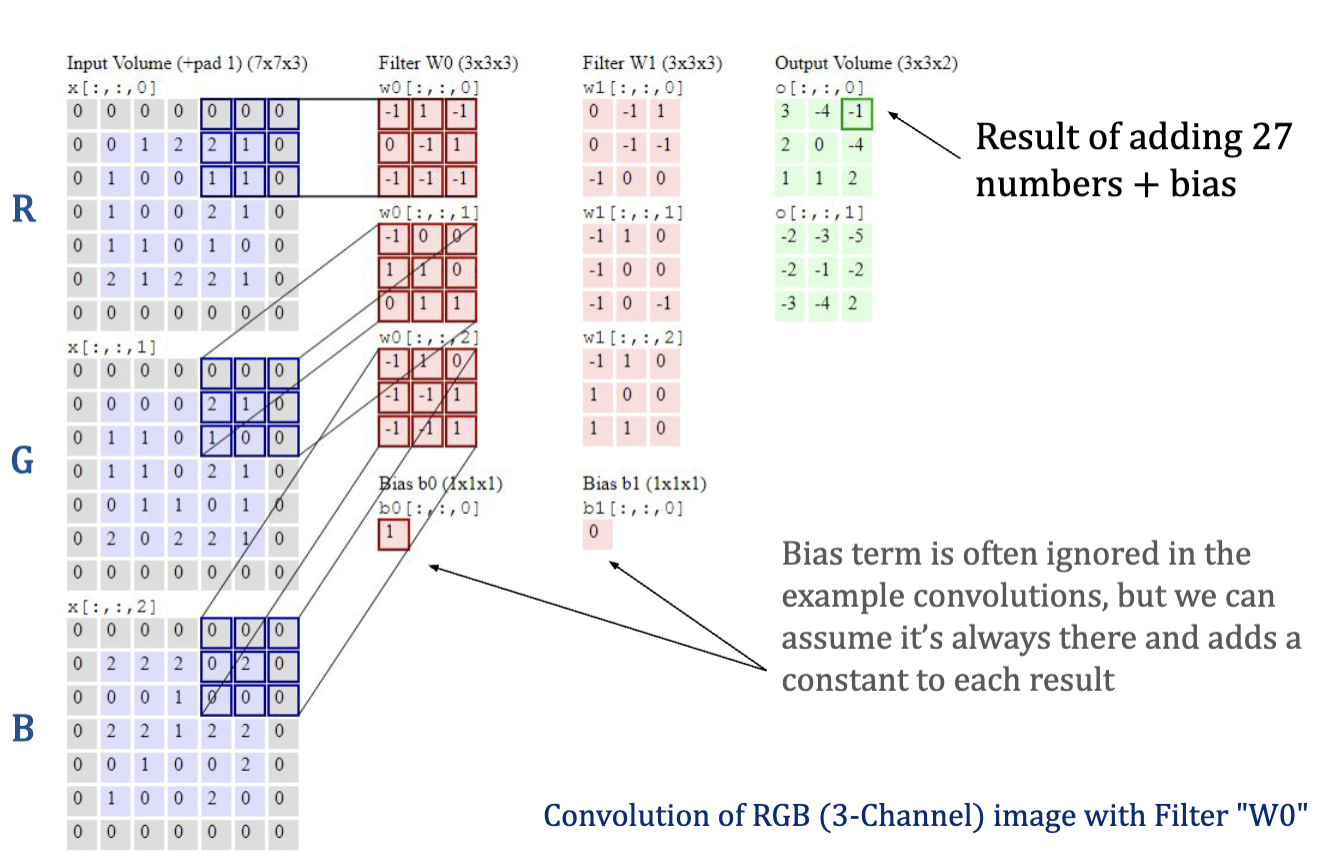
\includegraphics[width=0.75\linewidth]{Screenshot 2025-01-28 at 7.32.23 PM.png}
    \caption{Convolution of RGB (3-Channel) image with Filter W0}
    \label{fig:enter-label}
\end{figure}
Bias term is often ignored in the example convolutions, but can be assumed always there and adds a constant to each result.\\
Pink parameters are tunable. Have 2 of them to fulfill 2 channels needed for 2 layers.
\begin{enumerate}
    \item \textbf{How many input channels are there?}
    \begin{itemize}
        \item The input image has dimensions $3 \times 28 \times 28$, where the first dimension ($3$) represents the number of input channels (e.g., Red, Green, Blue for RGB images).
        \item \textbf{Answer:} There are \textbf{3 input channels}.
    \end{itemize}

    \item \textbf{How many output channels are there?}
    \begin{itemize}
        \item The convolution kernel has dimensions $5 \times 3 \times 8 \times 8$, where the first dimension ($5$) represents the number of output channels (one kernel per output channel).
        \item \textbf{Answer:} There are \textbf{5 output channels}.
    \end{itemize}

    \item \textbf{How many trainable weights are there?}
    \begin{itemize}
        \item Each convolution kernel has dimensions $3 \times 8 \times 8$, where:
        \begin{itemize}
            \item $3$ corresponds to the number of input channels.
            \item $8 \times 8$ is the size of the kernel.
        \end{itemize}
        \item The total number of weights per kernel is:
        \[
        3 \times 8 \times 8 = 192 \, \text{weights (per kernel)}.
        \]
        \item Since there are $5$ output channels, the total number of trainable weights is:
        \[
        5 \times 192 = 960 \, \text{weights}.
        \]
        \item \textbf{Answer:} There are \textbf{960 trainable weights}.
    \end{itemize}
\end{enumerate}
\subsection{Pooling Operator}
In a neural network with fully connected layers, we reduced the number of units before the final output layer. To be able to consolidate information, and remove information not useful for the current task.\\
Use strided convolutions, max pooling, average pooling.
\subsubsection{Max pooling}
pooling layers provide invariance to small translations of the input.
The size of output dimensions is computed by 
 \[
 o = \frac{i-k}{s}+1
 \]
\begin{itemize}
    \item Image dimension of size I
    \item Kernel of size k 
    \item Stride of size s
\end{itemize}
\paragraph{\textbf{Pros}:}
\begin{enumerate}
    \item \textbf{Feature Detection}:
    \begin{itemize}
        \item Captures the most prominent features (e.g., edges) within the window.
        \item Effective in reducing dimensionality while retaining essential spatial features.
    \end{itemize}
    \item \textbf{Non-Linear}:
Introduces non-linearity, which can help the model learn complex patterns.
    \item \textbf{Efficient}:
Reduces computational complexity by downsampling the feature map.
    \item \textbf{Better for ReLU Activations}:
Complements ReLU, as it focuses on the strongest activations, ignoring weaker ones.

\end{enumerate}
\paragraph{\textbf{Cons}:}
\begin{enumerate}
    \item \textbf{Information Loss}:
Discards information from non-maximal elements, which might be relevant in some contexts.
    \item \textbf{Overfitting}:
Can lead to overfitting for small datasets, as only the largest value is retained.
    \item \textbf{Sensitivity to Noise}:
Sensitive to outliers, as the maximum value might be a result of noise.

\end{enumerate}
 
\begin{figure}[H]
    \centering
    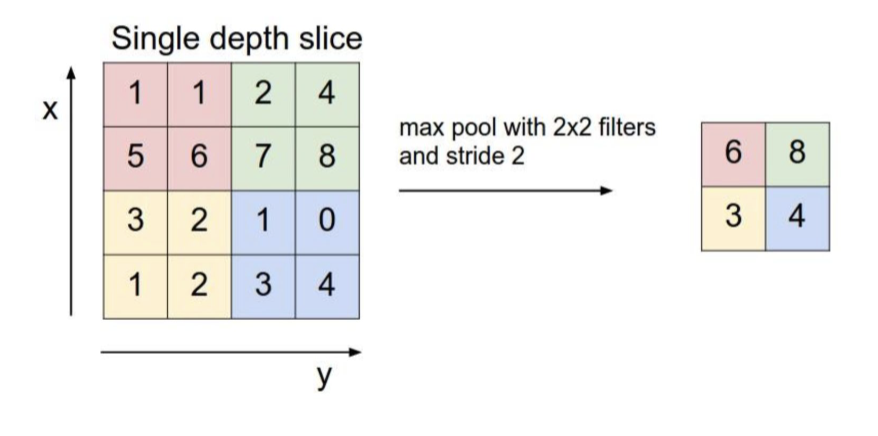
\includegraphics[width=0.5\linewidth]{Screenshot 2025-01-28 at 7.43.17 PM.png}
    \caption{Max Pooling}
    \label{fig:enter-label}
\end{figure}
\subsubsection{Average pooling}
Take average number of a frame of numbers and transpose them into a new matrix.
\paragraph{\textbf{Pros}:}
\begin{enumerate}
    \item \textbf{Smooth Feature Maps}:
Retains more general spatial information, which can be beneficial for tasks requiring smooth feature representations.
    \item \textbf{Robust to Noise}:
Less sensitive to outliers, as it considers all values within the window.
    \item \textbf{Stable Outputs}:
Leads to smoother feature maps, which may help when fine details are less important.

\end{enumerate}
\paragraph{\textbf{Cons}:}
\begin{enumerate}
    \item \textbf{Loss of Prominent Features}:
Dilutes the impact of strong activations by averaging them with weaker ones.
    \item \textbf{Less Effective in Feature Detection}:
Does not emphasize key patterns or activations as strongly as max pooling.
    \item \textbf{Higher Risk of Information Loss}:
While smooth, the averaging process might lose critical details.

\end{enumerate}

\subsubsection{Strided Convolution}
Shift the kernel by s when computing convolution instead of shifting by 1. This reduces the output parameters.
\paragraph{\textbf{Pros}:}
\begin{enumerate}
    \item \textbf{Simpler}:
Reduces the feature map size without requiring an explicit pooling layer.
    \item \textbf{Less Information Loss}:
Retains more spatial information compared to max pooling or average pooling.
    \item \textbf{Efficient}:
Reduces computations while avoiding additional operations like pooling.

\end{enumerate}
\paragraph{\textbf{Cons}:}
\begin{enumerate}
    \item \textbf{Less Focused}:
Does not emphasize prominent features (like max pooling).
    \item \textbf{Parameter Dependency}:
Effectiveness depends heavily on the choice of stride size.
    \item \textbf{No Additional Non-Linearity}:
Unlike max pooling, stride pooling does not introduce additional non-linear effects.

\end{enumerate}
 
\begin{figure}[H]
    \centering
    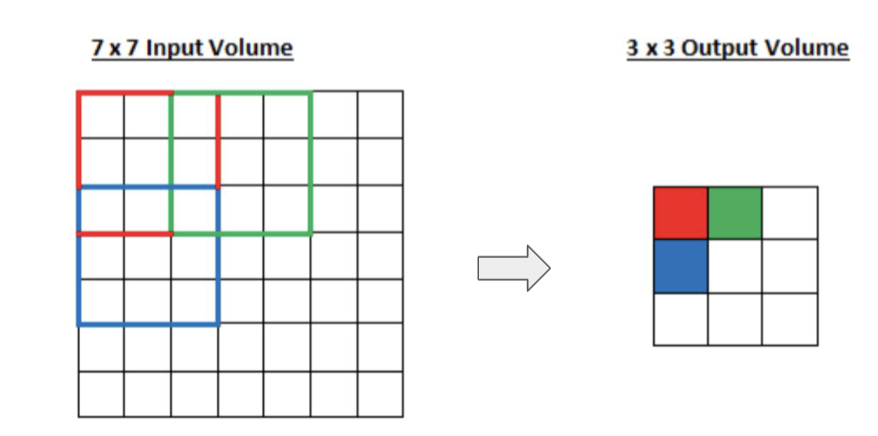
\includegraphics[width=0.5\linewidth]{Screenshot 2025-01-28 at 7.46.28 PM.png}
    \caption{Strided Convolution}
    \label{fig:enter-label}
\end{figure}
\subsection{Pytorch Implementation}
As we go through the CNN network layer by layer, the filter depth increases, the feature map height and width decrease.
\begin{figure}[H]
    \centering
    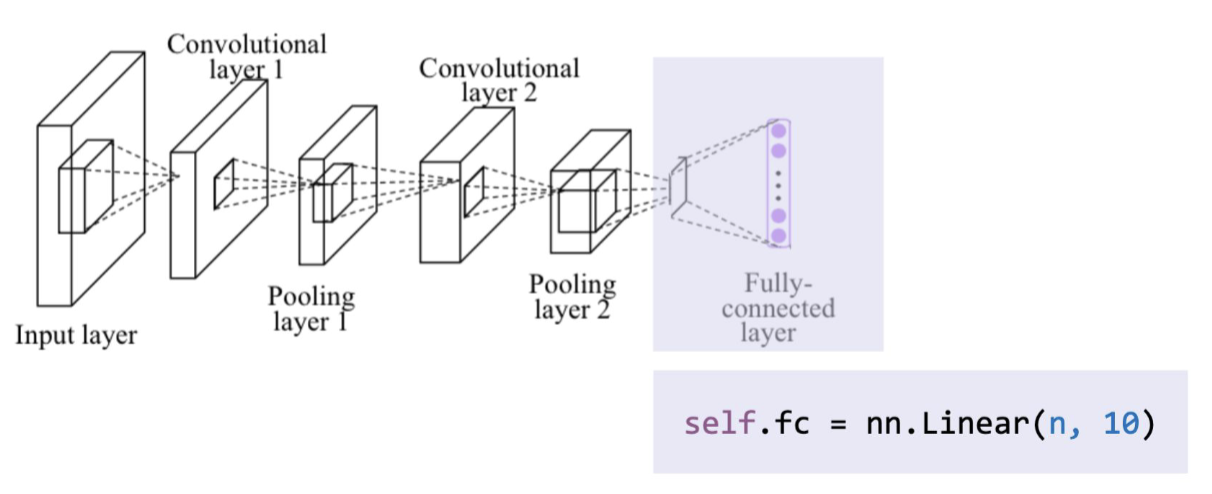
\includegraphics[width=0.75\linewidth]{CNN in Pytorch.png}
    \caption{Recall Linear}
    \label{fig:enter-label}
\end{figure}
(n,10), 10 output classes.
\begin{figure}[H]
    \centering
    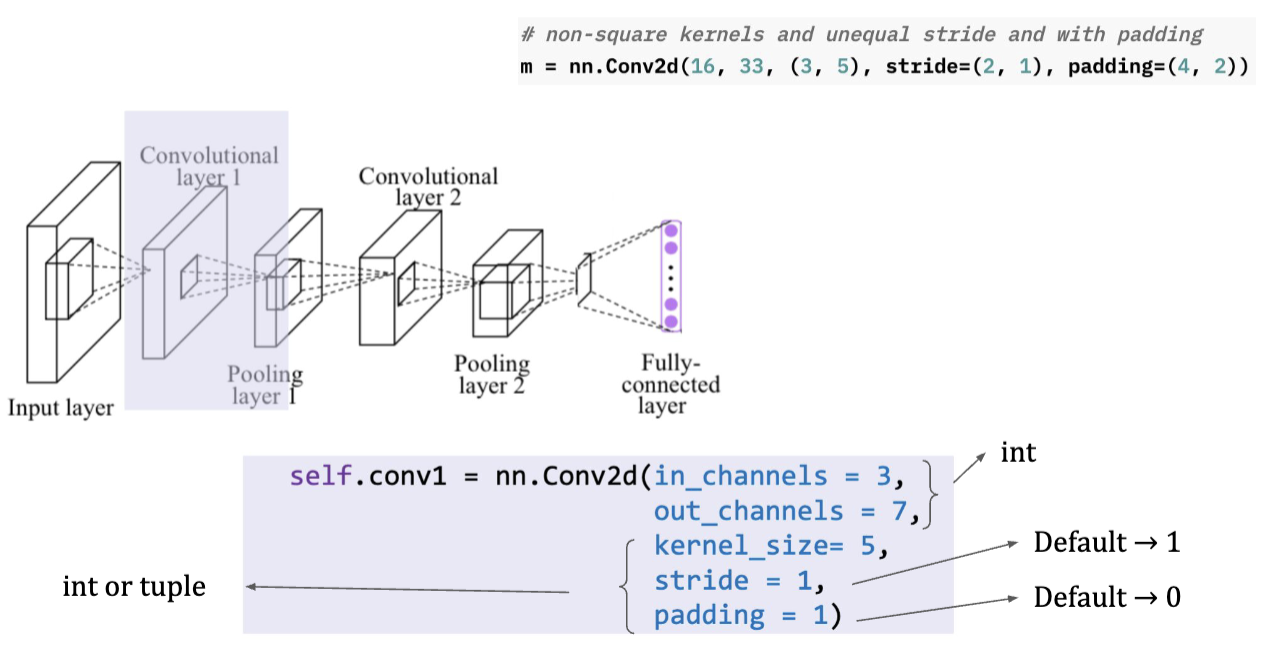
\includegraphics[width=0.75\linewidth]{Conv 2D.png}
    \caption{Conv 2D}
    \label{fig:enter-label}
\end{figure}
\begin{figure}[H]
    \centering
    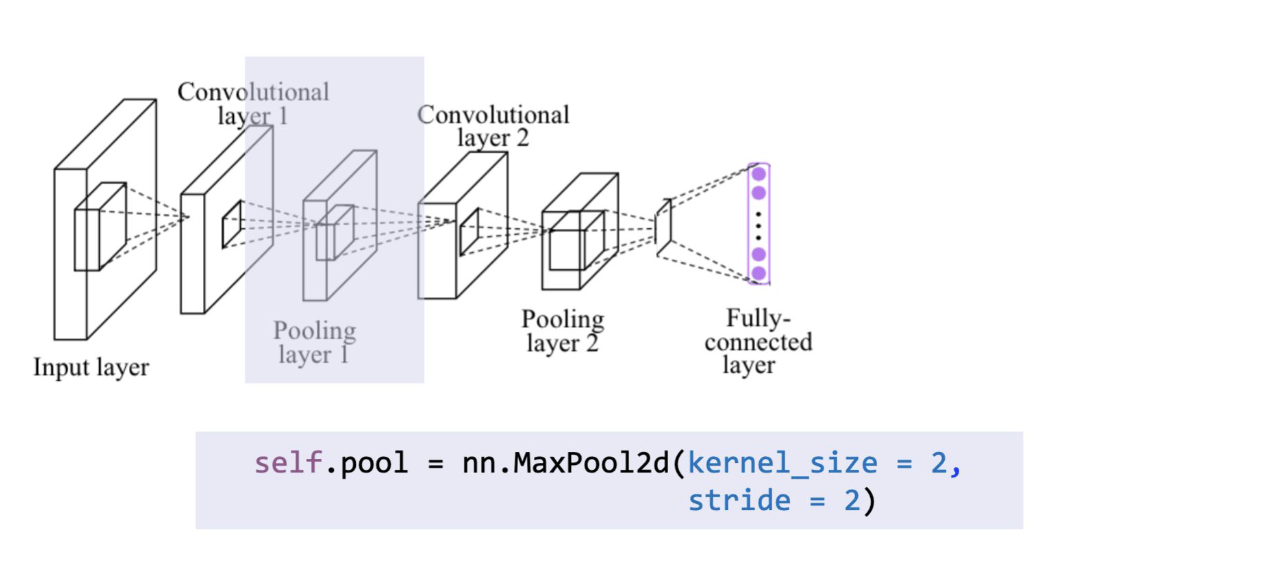
\includegraphics[width=0.75\linewidth]{MaxPool 2D.png}
    \caption{MaxPool 2D}
    \label{fig:enter-label}
\end{figure}
Sample Code
\begin{figure}[H]
    \centering
    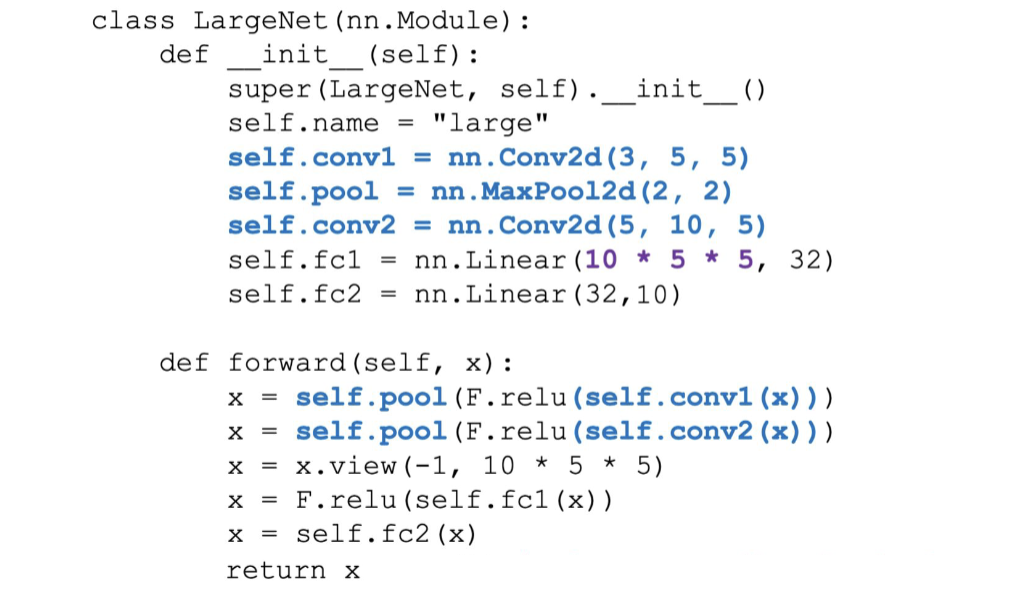
\includegraphics[width=0.75\linewidth]{CNN Sample Code.png}
    \caption{CNN Sample Code}
    \label{fig:enter-label}
\end{figure}
Only have 1 poling operator, weight needs to be distinct for sets of pooling operators. There is only one set of weight, therefore only one pooling operator.\\
Pooling is only defined once in the init method of the LargeNet class but is called multiple times during the forward pass because the pooling operation (self.pool) is reused. This approach avoids redundant definitions and promotes efficiency in the code.\\
There is no sigmoid activation function because it is built in the optimizer

\section{Midterm Review}
\subsubsection{2022Fall 4}
Implement a convolutional neural network with 3 convolutional layers and a single fully-connected layer which classifies the input image to one of the 100 classes. All convolutional layers use 3x3 kernels and stride of 2, and padding of 1. Starting from the input, the number of channels are [3, 8, 16, 32]. Suppose we use global average pooling to connect the feature maps to the fully-connected layer. Also suppose that we are using an intermediate classifier with the exact specifications of the final classifier over the second convolutional layer to provide more signal to the network. 
\begin{figure}
    \centering
    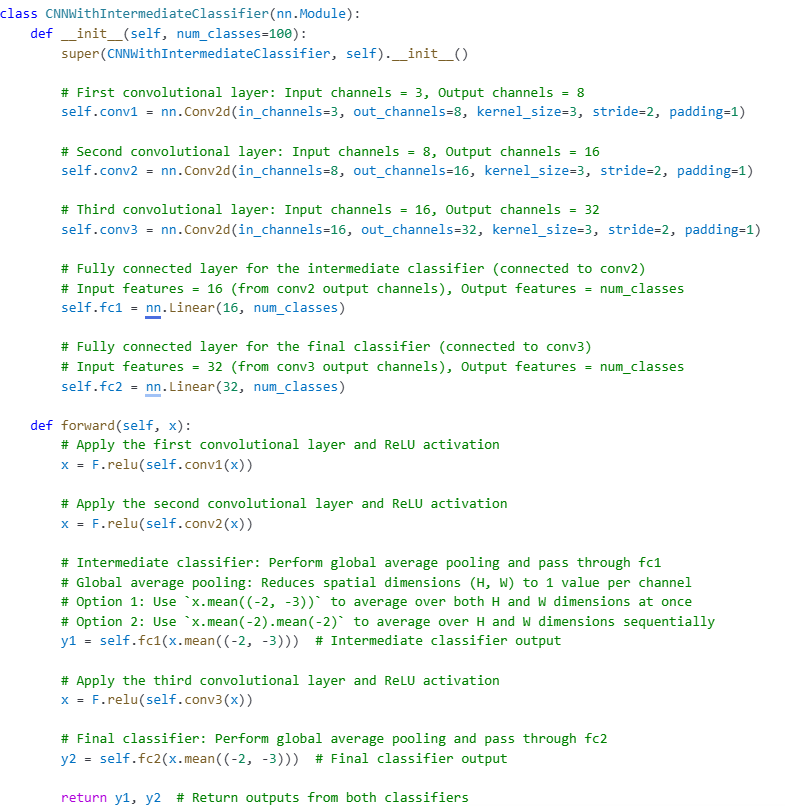
\includegraphics[width=1\linewidth]{question20224.png}
    \caption{Code}
    \label{fig:enter-label}
\end{figure}
\subsubsection{2022Fall 5}
Suppose we want to design an image search engine where given a query image we retrieve top 20 images from our image dataset ordered by their similarity to the query image. Also suppose that we have access to a pretrained ResNet model. Explain in details how you would implement this search engine. 

We use the pretrained model to extract the embeddings of all the images we have in dataset.
We use the same model to extract the embedding of the query image as well.
We then compare the embedding of the query image with all the embeddings in the database.
We sort the embeddings within the dataset based on their similarity to the query embedding and return the top 20 images corresponding to those embeddings.
\end{document}
